%%%%%%%%%%%%%%%%%%%%%%%%
% Sample use of the infthesis class to prepare an MSc thesis.
% This can be used as a template to produce your own thesis.
% Date: June 2019
%
%
% The first line specifies style options for taught MSc.
% You should add a final option specifying your degree.
% *Do not* change or add any other options.
%
% So, pick one of the following:
% \documentclass[msc,deptreport,adi]{infthesis}     % Adv Design Inf
% \documentclass[msc,deptreport,ai]{infthesis}      % AI
% \documentclass[msc,deptreport,cogsci]{infthesis}  % Cognitive Sci
% \documentclass[msc,deptreport,cs]{infthesis}      % Computer Sci
% \documentclass[msc,deptreport,cyber]{infthesis}   % Cyber Sec
% \documentclass[msc,deptreport,datasci]{infthesis} % Data Sci
% \documentclass[msc,deptreport,di]{infthesis}      % Design Inf
% \documentclass[msc,deptreport,inf]{infthesis}     % Informatics
%%%%%%%%%%%%%%%%%%%%%%%%

\documentclass[mphil,deptreport,ai]{infthesis} % Do not change except to add your degree (see above).
\usepackage[final]{pdfpages}

\begin{document}
\begin{preliminary}

\title{Spiking neural network model construction, inference, analysis and application}

\author{William Peer Berg}

\abstract{
%   Lorem ipsum. More computational power. More data, and higher res. data available. Modelling may (1) explain aspects about recorded site(s), and (2) generate hypotheses that may be tested with in vivo recording.
%   However, inference of high-dimensional biologically realistic (to some extent) models NP-hard, computationally costly, does not scale well with growing resolution due to dimensionality and cost, and not automated. Often experts are required to make an effort at hand-engineering models for particular data. As such, model inference of biologically realistic/plausible models is a highly challenging task, which if more automated might be of great benefit to the field of computational neuroscience.
%   Looking to machine learning and the success in applying gradient-based optimisation to tackle high-dimensional modelling problems, we here investigate the potential of applying this to the class of spiking neural network models. Further, we look at statistical assessment methods, and application of outlined methodology both to synthetically generated as well as biologically recorded in vivo data.
%   In sum, our results show that models may capture higher-order statistics of recorded nuclei, and that using some parallelisation tricks, we may decrease the computational cost to some extent. However, the lower bound on computational complexity still makes it challenging to apply the outlined methodology to very rich (i.e. high number of recorded nuclei) data sets.
SNNs biologically realistic models. Do we have the tools for SNN parameter inference, instead of rigorous and tedious hand-engineering?
ML advances: GBO.
SNNs differ from RNNs in a fundamental/crucial way. Show via parameter landscape and loss functions.
However, can find frontier(s).
SNN variants and applicability of GBO (only NLIF thus far, but still local minima).
To some extent GIF; frontier.
Same for GLIF versions??
Input scheme. Param landscape plots.
Loss functions.
PyTorch (+batching)

ABC, (EA; e.g. NGO)

Albeit GT off for the above, comparison wrt NMF.
Hand-engineered case and full analysis with NMF and LDA.

In conclusion...

BONUS (if time): Fitting to sleep data, with small sleep regul PPT/LDT lit rev first?

BONUS2: Append Izhikevich paper and place in context.

BONUS3: ?
}

\maketitle

\section*{Acknowledgements}
Arno.
Nina.
Patricia.
Luke.
Matthias.
Shuzo.

\tableofcontents
\end{preliminary}


\chapter{Introduction}


% The report then contains a bibliography and any appendices, which may go beyond
% page~40. The appendices are only for any supporting material that's important to
% go on record. However, you cannot assume markers of dissertations will read them.

% Citations (such as \cite{P1} or \cite{P2}) can be generated using
% \texttt{BibTeX}. For more advanced usage, the \texttt{natbib} package is
% recommended. You could also consider the newer \texttt{biblatex} system.

% You may not change the dissertation format (e.g., reduce the font
% size, change the margins, or reduce the line spacing from the default
% 1.5 spacing). Over length or incorrectly-formatted dissertations will
% not be accepted and you would have to modify your dissertation and
% resubmit.  You cannot assume we will check your submission before the
% final deadline and if it requires resubmission after the deadline to
% conform to the page and style requirements you will be subject to the
% usual late penalties based on your final submission time.

Spiking neural networks (SNNs) contain variables that represent biological properties such as membrane potential, temporal signature, and potentially ion channel dynamics. Their definition results in membrane voltage dynamics resembling that of biological neurons, including the release of action potentials upon reaching a certain membrane potential.
Due largely to the biological plausibility of this class of neural network models, they are appealing to study in computational neuroscience, as they may trail biology to a greater extent than the feed-forward networks as often seen in the machine learning domain.
However, training SNNs is yet of limited success, and model inference also faces a number of challenges due to the temporal constraints introduced by SNNs, as well as the increased complexity of this model class.
We here revisit the state-of-the art for inferring SNN models using both surrogate gradient based optimisation and some of the most prominent spike metrics, as well as deep neural network amortized learning and approximate Bayesian computation (ABC), and compare how these approaches may be employed for SNN inference. Further, we hypothesise that recent ML techniques may be leveraged for successful and efficient model inference using surrogate gradient descent.
We find that while ABC may be successful for population-level models, as has been shown recently in the literature, its algorithmic and computational complexity and cost thereof limits the methodology to a low number of nodes, particularly for more high-dimensional leaky integrate-and-fire (LIF) model extensions.
However, using a surrogate gradient approach, we find that model inference for larger networks is made possible. 
Since it would greatly help with SNN model construction if automatic inference based on various data became possible and available to the research community, this has been one of my primary research goals.
Further, as usual, more and more data, and data of a higher resolution, is becoming available from neural brain recordings, only increasing the potential benefits of developing a scalable approach for model inference.
We perform model inference using a set of LIF-extensions, leading up to the GLIF model using (both) synthetic (and biological) data, and demonstrate that higher order statistics may be captured (to some extent) even when performing neuron-level model inference over a mixed neuron-type network.
% This may advance research on SNN inference, and also demonstrates how modern ML frameworks as well as techniques may be leveraged to this end.
However, we observe that it is highly problematic to aim for retrieving ground-truth parameters in SNN models. A large part of the work presented in this thesis will revolve around why SNNs do not lend themselves as well as feedforward neural networks as within deep learning, even though they also implement a type of recurrence using recurrent units with memory, in addition to potential recurrent connectedness.
To try and give an intuition about why this is; if we think about deep neural networks (DNNs) in the machine learning (ML) domain - these may approximate arbitrary data well, given that they are universal function approximators. However, this requires that the data is of such a format that it may be represented and captured by a function which the network learns by spatial representation and transformation.
However, in the domain of SNNs, we introduce several new crucial properties, which results in distinct model dynamics. Each neuron now has a state, which depends on its previous state, and the behaviour is modelled typically as a system of ordinary differential equations (ODEs), containing parameters representing the membrane potential, membrane time constant relating to a refractory period, transmitter interaction, and other biological properties. 
While this makes the model biologically interpretable with direct parallels between parameters and biological and cellular counterparts, it also changes the entire system's behaviour.
The system now has activity inedpendently of input perturbation. The transformation of an input signal is no longer deterministic in the sense that it will result in one given output given a set of initial model parameters - it now depends on the current system's state, which again depends on the previous state.
As such, gradients calculated in a manner similar to that of for DNNs in ML will also depend on the system's and neurons' state, greatly increasing complexity.
In a way, one may still maintain the parallel to backpropagation through time for DNNs - however, there is a crucial difference in that a neuron's output is now of a much more binary nature; a spike or no spike, and in that the time series evolution of spikes, whilst potentially encoding much more information, now is a series of spike evolving over time, and thus the target signal cannot be regarded in the same way as in DNNs.
This being said, I believe like noted by other authors such as \cite{Sindaci2018StatisticalFunction} that researchers are looking for a connection between the field of machine learning and computational neuroscience, the former having had its subfield of DNNs created based on inspiration from the brain, but now in a reverse way in which we may leverage the advances from the domain of ML in model construction.
Even though we are not there yet, I believe the search for a connection here may both be highly beneficial for the community, and spawn a new sub-field of dynamical systems modelling using inference in computational neuroscience.

My main findings, although included throughout in the rest of my thesis, may be summarised as following:
\subsection{SNNs are hard to optimise}
I am starting to believe that they’re in fact not possible to optimise, due to the parameter landscape, which results from the temporal nature of the target signal.
In DNNs, we only consider approximating a spatial transformation over the input data. Not only does this allow for higher parallelisation of the training algorithm, but it may also greatly constrain the parameter landscape in the sense that it does not depend on the past activity of the network itself, which vastly increases both the complexity and stochasticity of parameter inference. 
One way to ameliorate this is to eliminate some of the stochasticity by making the neurons non-leaky. Since we may computationally set the system’s initial conditions and random seed, the following deterministic computations have little to no fluctuations, and with no leakage, gradient propagation may be computed exactly according to the error signal.

\subsection{Another issue of SNNs is the binary output signal}
One way of addressing this issue is by incorporating the signal below spike-threshold, i.e. the membrane potential, and have this generate a signal inside of an active zone, such as when the potential is above 0. This is not entirely biologically unrealistic, …, and it offers the advantage of a continuous signal centred around potential (no pun intended) spike pulses, or action potentials. Note that it also provides a gradient signal for spike generation even when the potential may be below threshold, still making the excitation visible to the optimiser.
This bears some resemblance to loss metrics such as the van Rossum distance, in which each spike pulse is convolved with an exponentially decaying kernel, such that we may operate over a smoother signal. However, this signal transformation transforms each spike pulse the same, rendering the sub-threshold gating synapse model a more fine-grained candidate, since it contains richer differentiable information, and not just spike-time information.

\subsection{Multiple local minima - no well-defined global optimum}
Even when addressing the issues above with the proposed approaches, and even if fixing all model parameters but the weight matrices, there are multiple weight configurations that may result in very similar behaviour and outputs.
As noted by other researchers in the DNN as well as SNN literature (...) the initial configuration has a large effect on the resulting inferred weights and/or model. This holds particularly true for SNNs, where the previous model state also has an effect on the future state, and the model neurons may be brought to exert different modes of behaviour, depending on the previous and current input and state.

\subsection{Hand-engineered models may be qualitatively similar local minimum}
By hand-engineering models it is possible to attain qualitative patterns and behaviour, which has been a common practice in the field of comp neuro - however, this may not be satisfactory for attaining higher-order statistics, and requires a large amount of resources. Therefore, model inference may likely be a better option. 
The above however indicates that GLMs may be the best we can do in this regard (wrt spike trains), and demonstrates a need for advancing SNN inference.
The way going forward?
Amortised learning provides a posterior over the parameters.
However, it quickly becomes intractable due to the high complexity of models.
Surrogate or exact gradient approaches are difficult due to aforementioned issues, and most likely do not settle into a stable configuration, as well as stay in planes of local minima.
These findings suggest that the best we can currently do is using approximate Bayesian approaches, which not only lets us infer a posterior over all of the parameters, but also provides a measure of certainty around the parameters.

Temmporary conclusion:
If this approach is intractable for the case we’re looking at, the best we may do is either to use other information theoretic approaches to assess whichever aspect it is that we are interested in, including potentially to hand-engineer and rigorously test a proposed model.


\chapter{Spiking neural network models}

\section{Models}

\subsection{LIF}

\subsection{GLIF}

\subsection{Izhikevich}
\subsubsection{Contribution: Izhikevich recovery variables work (?)}

\subsection{GIF}

\subsection{NLIF}


\section{The link to recurrent neural networks}


\section{Optimisation}
\cite{Taherkhani2020} learning in SNNs

\subsection{Contribution: PyTorch}

\subsection{Contribution: Batching and SNNs}

\subsection{Contribution: Loss metrics comparison}

\subsection{Contribution: LIF paper}
% 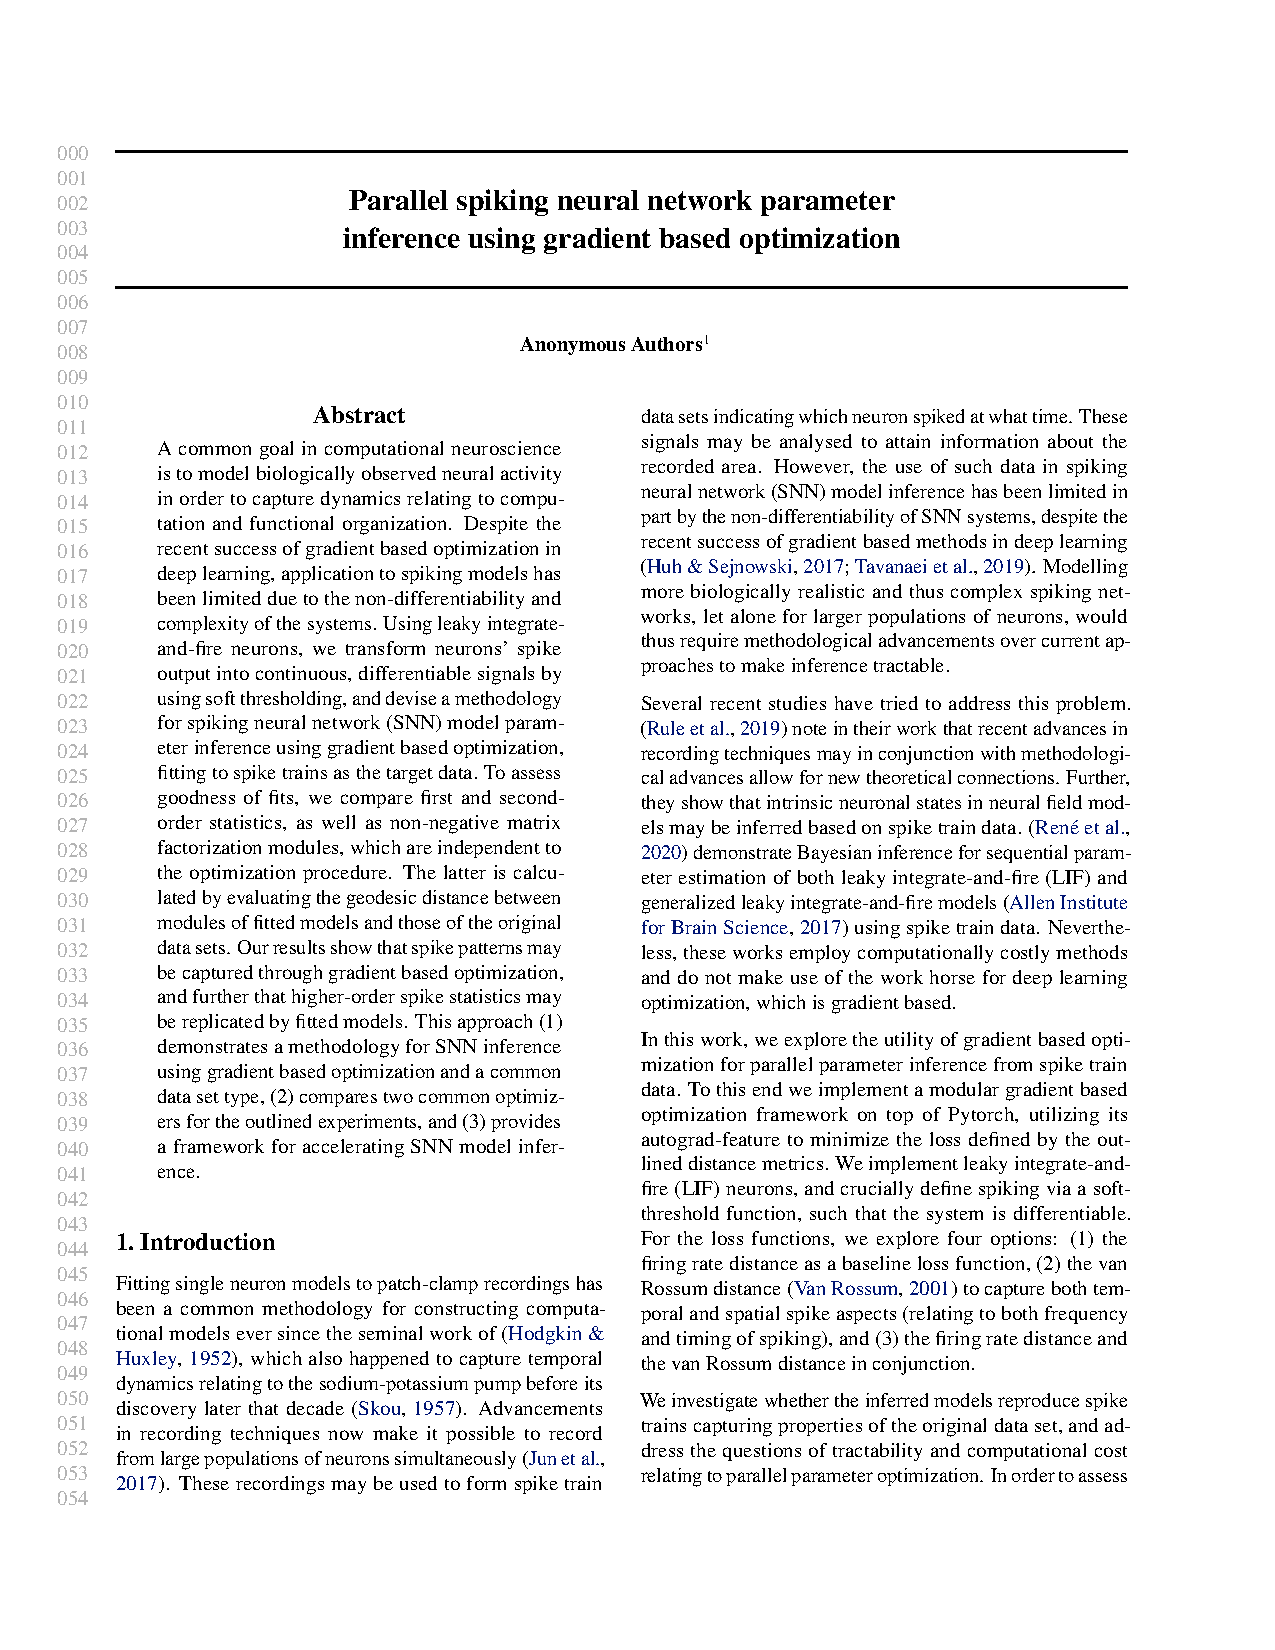
\includepdf[pages=-]{files/icml2021_draft_snn_inference.pdf}

\subsection{Contribution: Stochasticity and SNNs}

\subsection{Contribution: NLIF work}

\subsection{Contribution: microGIF work}


\section{Bayesian approaches}

\subsection{MCMC sampling}
\cite{Rene2020} "special case" i.e. mesoscopic-microscopic inference using first ABC (or GD?) on pop. level and then MCMC sampling for full approx. posterior?

\subsection{Amortised learning with DNNs}
\cite{Lueckmann2018} amortised learning and ABC using DNNs.

% \section{Evolutionary algorithms}


\section{Analysing SNNs}

\subsection{NMF}

\subsection{LDA}

\subsection{Generalised Linear Models}



\chapter{Sleep regulation in the rodent brainstem}

My initial research proposal outlines a research project where the goal is to meet research needs within the field of sleep regulation through computational modelling.
More specifically, the aspiration was to model neurons of the pedunculopontine and laterodorsal tegmental areas within the brainstem during different brain states, based on their neuroanatomy as described, even though scarcely, within the literature, and based on in vivo data from these brain areas \cite{Herice2019c, Tsunematsu2019, Pal2007, Martinez-Gonzalez2011, Fraigne2015}.
Further, an overarching research goal was to be able to capture the emergence of neural ensembles as identified in vivo in the model by using non-negative matrix factorisation (NMF) \cite{Seung1999, Seung2001, Onken2016a}.
Computational modelling and spiking neural network (SNN) inference covers several research needs within the field of sleep research and the synthesis of neuroscience and its computational counterpart in that it addresses model scarcity, as well as a methodology for accelerating modelling by inference through gradient-based optimisation \cite{Herice2019c, Huh2017, Taherkhani2020}.
This was the foundation for sparking my interest in a methodological project in which we seek to automate biologically relevant neural network model inference, and more specifically to research both (1) the current state-of-the-art on SNN inference, and (2) leveraging ML based methods of gradient descent and optimisation for SNN inference \cite{Huh2017, Mostafa2020, Tavanaei2019b, Lee2016}.

\section{Analysis of data}

\section{Inference}

\subsection{GBO}

\subsection{ABC}

\subsection{Comparison and conclusion}





\bibliographystyle{plain}
\bibliography{references}

%% You can include appendices like this:
% \appendix
% 
% \chapter{First appendix}
% 
% \section{First section}
% 
% Markers do not have to consider appendices. Make sure that your contributions
% are made clear in the main body of the dissertation (within the page limit).

\end{document}
